% CVPR-style template
\documentclass[10pt,twocolumn,letterpaper]{article}

\usepackage[pagenumbers]{cvpr}
\usepackage{graphicx}
\usepackage{subcaption}
\usepackage{amsmath}
\usepackage{amssymb}
\usepackage{booktabs}
\usepackage{array}
\usepackage{tabularx}
\usepackage[table,dvipsnames]{xcolor}
\usepackage{xeCJK}
\setCJKmainfont{Noto Serif CJK TC}
\usepackage[pagebackref,breaklinks,colorlinks]{hyperref}
\usepackage[capitalize]{cleveref}
\crefname{section}{Sec.}{Secs.}
\Crefname{section}{Section}{Sections}
\crefname{table}{Tab.}{Tabs.}
\Crefname{table}{Table}{Tables}
\crefname{figure}{Fig.}{Figs.}
\Crefname{figure}{Figure}{Figures}

\begin{document}

\title{\LARGE HW4: Image Restoration Report \\[0.5em] \large Visual Recognition using Deep Learning, NYCU}
\author{朱驛庭, 111550093}
\maketitle

\section{Introduction}
\label{sec:intro}

This work tackles the HW4 all-in-one image restoration task. The training set contains 1{,}600 rain-degraded/clean pairs and 1{,}600 snow-degraded/clean pairs, while the test set contains 100 degraded images whose degradation type is hidden. The metric is PSNR, and the constraints are strict: a single PromptIR-based model must handle both rain and snow, no external data is allowed, and all weights must be trained from scratch.

I build the solution on PromptIR~\cite{potlapalli2023promptir}, a Restormer-style all-in-one restoration network. The final submitted model modifies PromptIR with a SimpleGate feed-forward module, frequency-aware AdaIR-style prompt generation, Charbonnier plus frequency-domain losses, exponential moving average (EMA) weights, larger crops, longer training, and D4 test-time augmentation. The best public submission is \textbf{31.51 PSNR}, corresponding to public leaderboard rank 26 under team name \texttt{chueating}. The project repository is available at \url{https://github.com/ChuEating1005/VRDL/tree/main/HW4}.

\section{Method}
\label{sec:method}

\subsection{Data Preprocessing and Augmentation}
All images were verified to be RGB images of size $256\times256$. For training, each degraded image is paired with its corresponding clean image by filename: \texttt{rain-i.png} with \texttt{rain\_clean-i.png}, and \texttt{snow-i.png} with \texttt{snow\_clean-i.png}. No external data or pretrained weights are used.

During training, I sample paired random crops and apply only restoration-safe geometric augmentation: horizontal flip, vertical flip, and random 90-degree rotations. The final model uses crop size $192\times192$ and batch size 4. At inference time, predictions are clipped to $[0,1]$, converted to uint8, and stored in the required \texttt{pred.npz} format with keys \texttt{0.png}--\texttt{99.png} and arrays of shape $(3,H,W)$.

\subsection{PromptIR Backbone}
PromptIR~\cite{potlapalli2023promptir} is designed for all-in-one image restoration. Its backbone follows Restormer~\cite{zamir2022restormer}: an encoder-decoder transformer with overlapping patch embedding, multi-Dconv head transposed attention (MDTA), gated-Dconv feed-forward networks (GDFN), skip connections, and multi-scale refinement. MDTA computes channel attention instead of full spatial attention, which keeps the model efficient for high-resolution restoration. GDFN combines point-wise expansion, depth-wise convolution, a nonlinearity gate, and projection to model local and channel-wise interactions.

The core contribution of PromptIR is the \textbf{Prompt Block}. Instead of requiring explicit degradation labels, the network learns a bank of prompt components. For an input feature, global average pooled statistics produce softmax weights over the prompt bank; the weighted prompt is then resized and fused into decoder features. This gives the network an input-conditioned hint about what degradation is present. This design fits HW4 because the test filenames do not reveal whether an image contains rain or snow; the model must infer degradation type internally.

\subsection{Architecture Modifications}
The final model, denoted \textbf{v3}, keeps PromptIR as the base model but modifies two components.

\paragraph{SimpleGate FFN.} Inspired by NAFNet~\cite{chen2022nafnet}, I replace the original GELU-style gate in the feed-forward network with a SimpleGate: after expansion, the feature channels are split into two halves and multiplied element-wise. This removes the explicit activation while preserving multiplicative feature selection. The hypothesis is that restoration benefits from simple, low-overhead gating because the target mapping is mostly low-level and pixel-accurate rather than semantic.

\paragraph{Frequency-aware AdaIR prompt.} I additionally implement an AdaIR-style prompt generator~\cite{cui2024adair}. Decoder features are decomposed in the Fourier domain into low- and high-frequency components using \texttt{rfft2}. The two bands route through separate prompt banks and are fused by a learned channel gate. The motivation is that rain streaks are dominated by high-frequency directional structures, while snow contains both high-frequency flakes and lower-frequency haze/occlusion. Frequency-conditioned prompts should therefore provide a better degradation cue than a single prompt bank.

The final v3 model has \textbf{37.97M parameters}, compared with 35.59M for the original copied PromptIR implementation.

\subsection{Optimization and Hyperparameters}
All models are trained from scratch with AdamW~\cite{loshchilov2019adamw}, learning rate $2\times10^{-4}$, cosine decay, 8 warmup epochs for v3, AMP mixed precision, and gradient clipping disabled. The validation split is 5\% of the training pairs. The final v3 training recipe uses 200 epochs, batch size 4, crop size 192, and EMA decay 0.999.

The loss combines Charbonnier loss and a frequency-domain L1 loss:
\[
\mathcal{L}=\sqrt{(\hat{x}-x)^2+\epsilon^2}+0.1\,\|\mathcal{F}(\hat{x})-\mathcal{F}(x)\|_1,
\]
where $\epsilon=10^{-3}$ and $\mathcal{F}$ is the real 2D Fourier transform. The FFT loss follows the intuition of frequency-domain restoration methods such as FFTformer~\cite{kong2023fftformer}: rain and snow artifacts are visible in the spectrum, so matching only pixels may under-penalize structured residual streaks or flakes.

\subsection{Inference and Ensembling}
For the final submission, I use D4 test-time augmentation with eight transforms: four rotations times optional horizontal flip. Each restored output is inverse-transformed and averaged in floating point before uint8 conversion. I also tested prediction-level ensembles across different runs. Since v2/v3/v4 do not always share identical prompt modules, I ensemble restored images rather than averaging checkpoint weights.

\section{Experiments and Results}
\label{sec:results}

\subsection{Main Results}
\Cref{tab:main_results} summarizes validation and public leaderboard performance. The final v3 model reaches 30.648 validation PSNR and 31.51 public PSNR with TTA-8. It improves over the baseline by +1.02 validation PSNR and +1.46 public PSNR over the baseline TTA submission.

\begin{table*}[t]
\centering
\scriptsize
\setlength{\tabcolsep}{4pt}
\renewcommand{\arraystretch}{1.12}
\begin{tabularx}{\textwidth}{@{}>{\raggedright\arraybackslash}p{0.14\textwidth}>{\raggedright\arraybackslash}X>{\centering\arraybackslash}p{0.08\textwidth}>{\centering\arraybackslash}p{0.08\textwidth}>{\raggedright\arraybackslash}p{0.20\textwidth}@{}}
\toprule
Run & Main setting & Val PSNR & Public PSNR & Notes \\
\midrule
Baseline no TTA & PromptIR, L1, crop 128, 120 ep & 29.628 & 29.81 & Original PromptIR copied verbatim \\
Baseline TTA & Same baseline + flip/rotation TTA & 29.628 & 30.05 & TTA gives +0.24 public PSNR \\
v4 no TTA & SimpleGate + Charbonnier + FFT + EMA & 30.120 & 30.08 & Base Prompt Block \\
v4 TTA-8 & v4 + D4 TTA & 30.120 & 30.31 & +0.23 over no TTA \\
v2 TTA-8 & v4 + AdaIR prompt, crop 128, 120 ep & 29.825 & 30.26 & AdaIR under-trained here \\
\rowcolor{Yellow!18} v3 TTA-8 & v2 architecture, crop 192, 200 ep & \textbf{30.648} & \textbf{31.51} & Best single model \\
v2+v3+v4 ensemble & Prediction average of TTA-8 outputs & -- & 30.91 & Worse than v3 alone \\
\bottomrule
\end{tabularx}
\caption{Validation and public CodaBench results. Public scores are from the submitted zip files shown in the provided submission screenshot.}
\label{tab:main_results}
\end{table*}

\subsection{Additional Experiments}
The homework explicitly asks for innovative ideas or additional experiments beyond pure hyperparameter tuning. I therefore focus on architectural, loss, and inference changes, each with a hypothesis, result, and implication.

\paragraph{Experiment 1: SimpleGate + Charbonnier/FFT + EMA.} The hypothesis was that low-level restoration benefits from simpler multiplicative gating, robust pixel loss, explicit frequency supervision, and smoothed weights. Replacing baseline L1 PromptIR with this combined recipe (v4) improved validation PSNR from 29.628 to 30.120 and public TTA score from 30.05 to 30.31. This supports the idea that rain/snow restoration is not only a backbone problem; optimization target and stable averaging are important.

\paragraph{Experiment 2: AdaIR frequency-aware prompting.} The initial hypothesis was that separating low- and high-frequency prompt routing would help distinguish rain streaks and snow structures. At crop 128 and 120 epochs, this was false: v2 reached only 29.825 validation PSNR, 0.30 below v4. However, when the same AdaIR architecture was trained with larger 192 crops and 200 epochs, v3 reached 30.648 validation PSNR and 31.51 public PSNR. The implication is compute-budget dependent: AdaIR's extra capacity is harmful when under-optimized, but becomes the best model once the crop exposes larger frequency patterns and the optimization horizon is long enough.

\paragraph{Experiment 3: D4 test-time augmentation.} The hypothesis was that image restoration should be approximately equivariant to rotations and flips, while the trained network is not perfectly equivariant. TTA improved the baseline public score from 29.81 to 30.05 and v4 from 30.08 to 30.31. This confirms TTA as a reliable inference-time improvement. However, prediction averaging across heterogeneous models did not always help: the v2+v3+v4 ensemble scored 30.91, below v3's 31.51, likely because weaker models over-smoothed details restored correctly by v3.

\subsection{Training Curves}
\Cref{fig:curves} shows the WandB screenshots used to monitor training. v4 converges around 120 epochs, while v3 continues benefiting from the longer schedule and larger crop. EMA and online validation scores are close near convergence, suggesting that cosine LR already smooths the late trajectory.

\begin{figure*}[t]
  \centering
  \begin{subfigure}[t]{0.32\linewidth}
    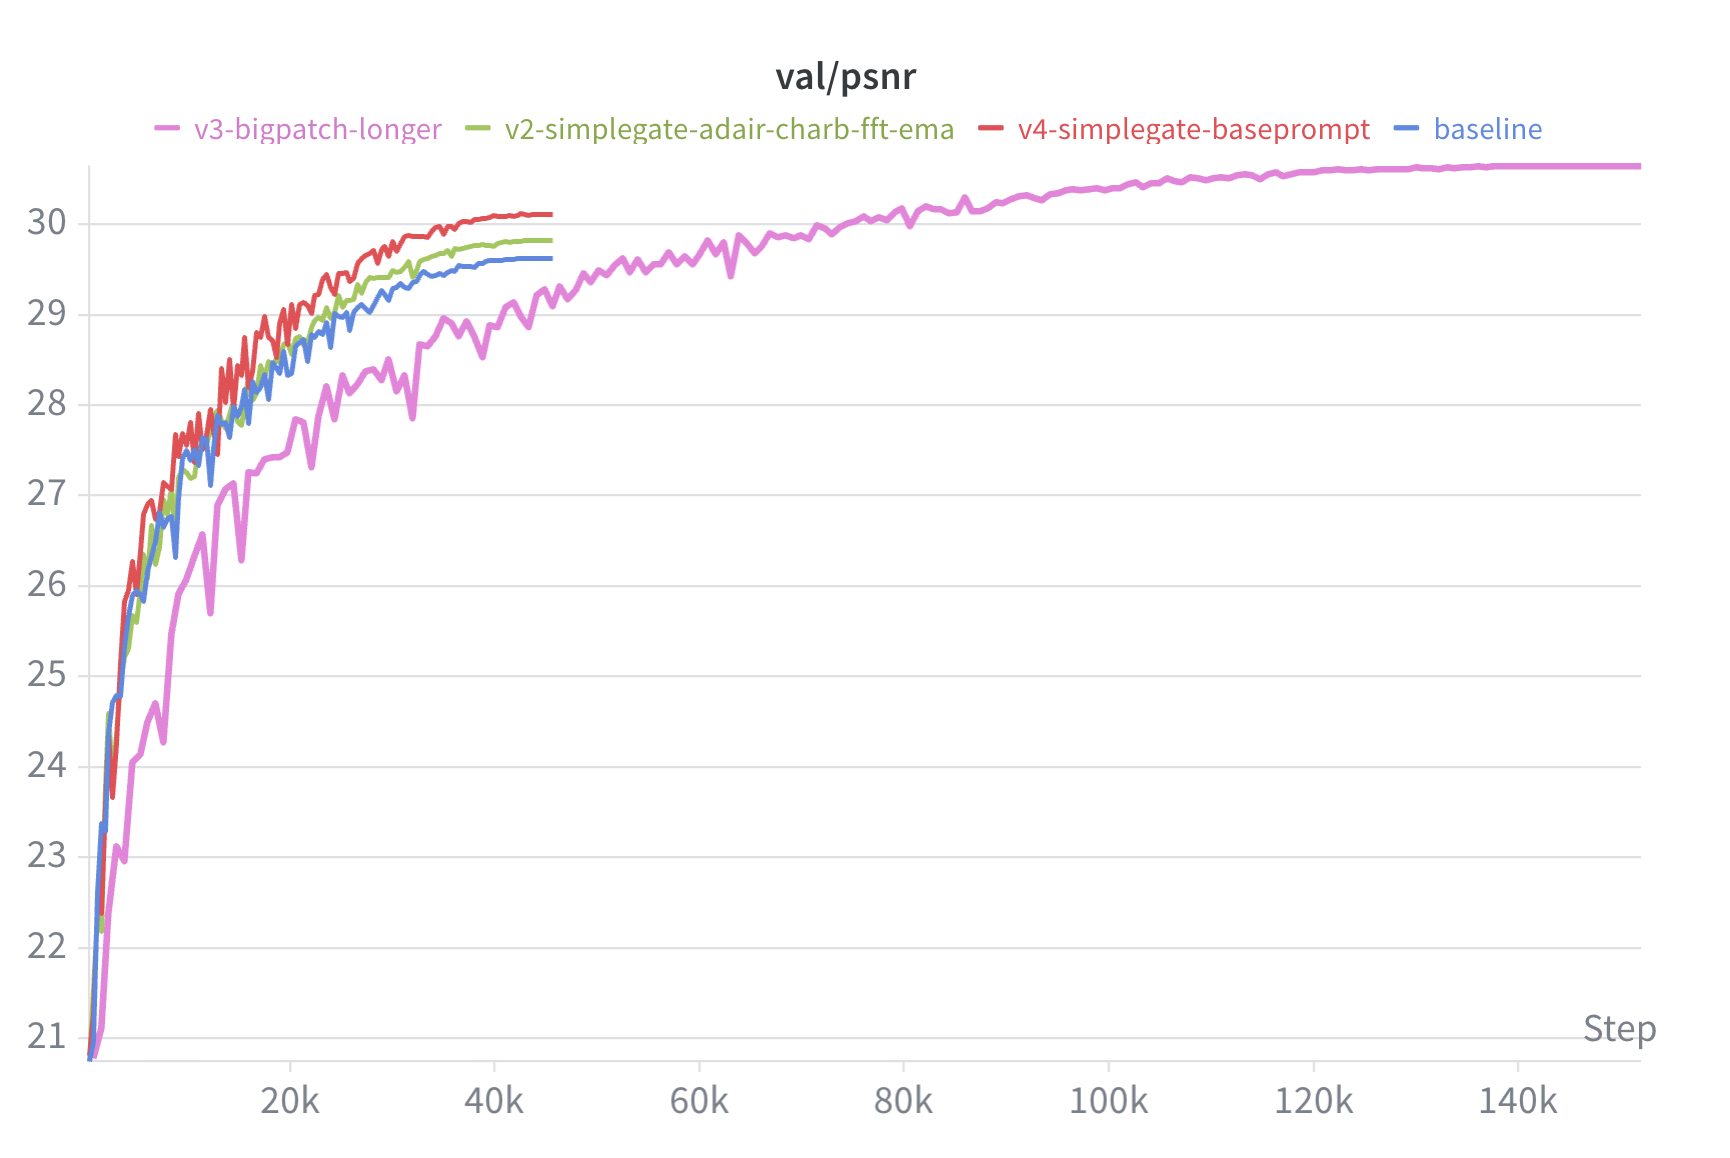
\includegraphics[width=\linewidth]{assets/val_psnr.png}
    \caption{Validation PSNR (online vs.\ EMA).}
  \end{subfigure}
  \hfill
  \begin{subfigure}[t]{0.32\linewidth}
    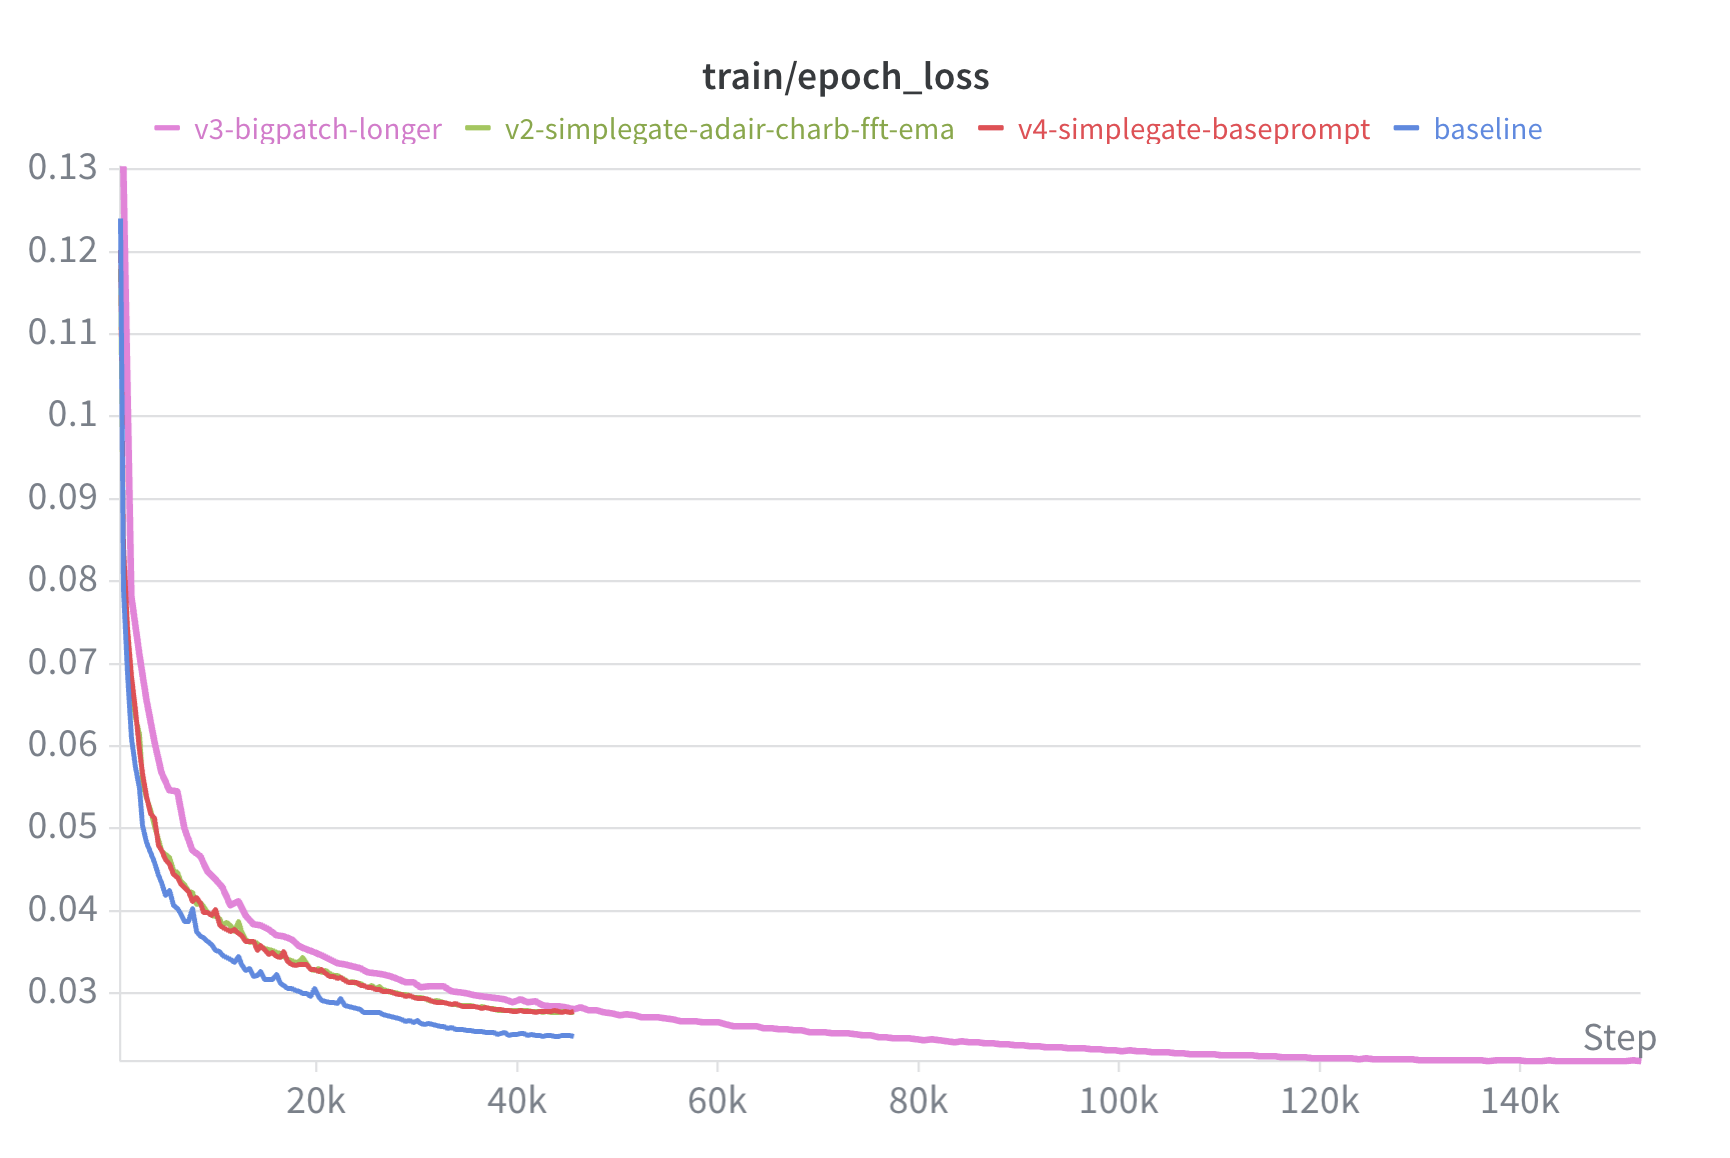
\includegraphics[width=\linewidth]{assets/train_epoch_loss.png}
    \caption{Per-epoch training loss (Charbonnier + 0.1$\cdot$FFT).}
  \end{subfigure}
  \hfill
  \begin{subfigure}[t]{0.32\linewidth}
    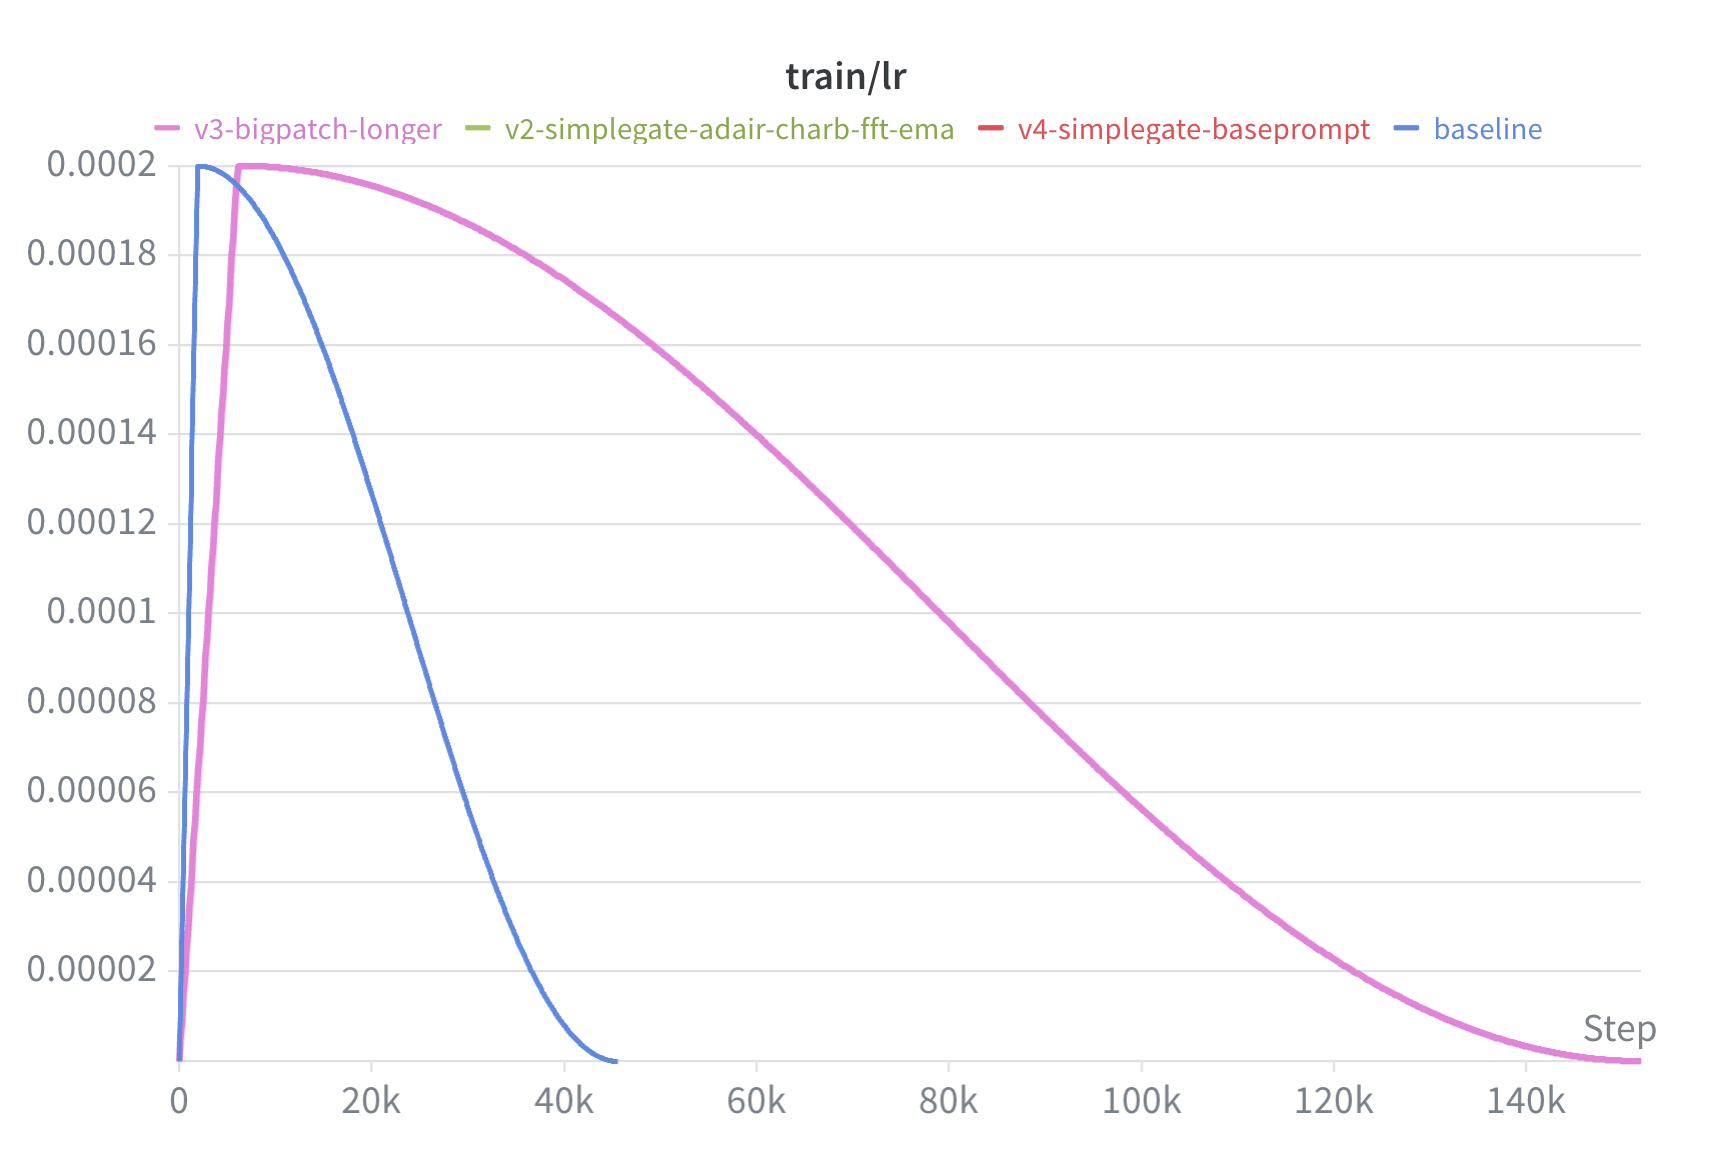
\includegraphics[width=\linewidth]{assets/train_lr.png}
    \caption{Cosine learning-rate schedule with linear warmup.}
  \end{subfigure}
  \caption{WandB training curves for the three main runs (v2, v3, v4).}
  \label{fig:curves}
\end{figure*}

\section{Conclusion}
The final solution satisfies all HW4 constraints: it uses PromptIR as the required model, trains from scratch, uses no external data, and submits a single model output file in the required \texttt{pred.npz} format. The strongest result is v3 with 31.51 public PSNR. The main finding is that PromptIR's prompt mechanism can be strengthened by frequency-aware prompting, but only when the training crop and schedule provide enough context and optimization budget. TTA is a robust final improvement, while ensembling with weaker models can reduce PSNR by over-smoothing outputs.

GitHub repository: \url{https://github.com/ChuEating1005/VRDL/tree/main/HW4}.

{\small
  \bibliographystyle{ieee_fullname}
  \bibliography{egbib}
}

\end{document}
